\capitulo{5}{Aspectos relevantes del desarrollo del proyecto}

\section{Arquitectura del Player}
Player es el GameObject asociado al avatar que controlará el jugador y posee un componente PlayerController. La clase PlayerController, se encarga del funcionamiento del objeto como avatar controlable por el jugador.

La clase PlayerController hereda de la clase KinematicObject. KinematicObject es una clase que hereda de MonoBehaviour y se encarga de simular la gravedad sobre el objecto y gestionar las colisiones contra obstáculos que puedan afectar al movimiento (se profundizará en este aspecto en el apartado de gestión de las colisiones).

\clearpage
\begin{figure}[h]
\centering
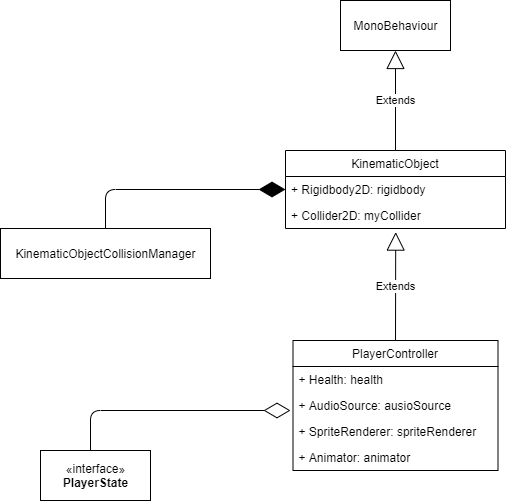
\includegraphics[scale=0.7]{Memoria/Aspectos_relevantes/Arquitectura_Player/Jerarqui_herencia_PlayerController}
\caption{Jerarquía de herencia de PlayerController}
\end{figure}

El PlayerController utiliza elpatron de diseño Estado, de manera que hay acciones generales que realiza la propia clase PlayerControler y otras que delega en las clases que heredan de la interfaz PlayerState
Las operaciones generales que realiza PlayerController son:
\begin{itemize}
\item
Para el método Update se encarga de la animación del personaje (de la parte más genérica) y de comprobar si algún botón o tecla asociado a una acción ha sido pulsado y se requiere alguna acción como respuesta (esa acción se ejecutará en el FixedUpdate).
\item
Para el método FixedUpdate se actualizan las banderas y en caso de haber pulsado el botón de salto o del acelerón se realiza la acción (si se puede realizar). Las banderas son una serie de variables booleanas que marcan si se pueden o no realizar acciones concretas. Las banderas son los booleanos que dictaminan si se puede o no ejecutar las mecánicas del Player.
\end{itemize}

\subsection{Estados del Player}
Los estados que utiliza PlayerController son una aplicación del patrón de diseño Estado que modificará el comportamiento del Player. Se ha tomado esta decisión porque las operaciones a realizar por PlayerController variarán en función de en qué situación se encuentre. Las situaciones en las que se encontrará el Player pueden cambiar en tiempo de ejecución y obligarán a realizar operaciones distintas.

A continuación se mostrará un diagrama con los posibles estados y las condiciones permiten pasar de uno a otro:

\clearpage
\begin{figure}[h]
\centering
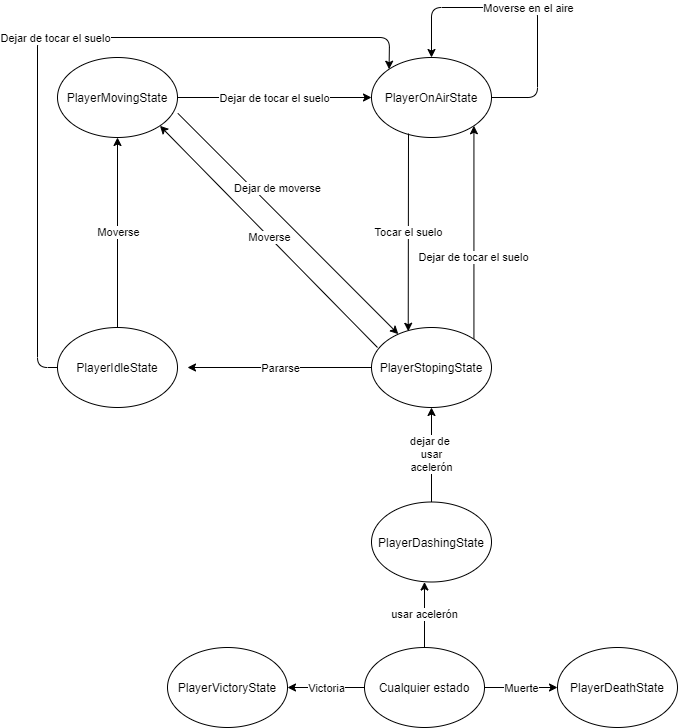
\includegraphics[scale=0.6]{Memoria/Aspectos_relevantes/Arquitectura_Player/Diagrama_de_estados}
\caption{Diagrama de transición entre estados de PlayerController}
\end{figure}

Todos los estados heredan de la interfaz PlayerState, que implementa los métodos UpdateState y FixedUpdateState. UpdateState será llamado en el método Update de PlayerController y FixedUpdateState será llamado por el método FixedUpdate de PlayerController. Los estados realizan las siguientes operaciones:
\begin{itemize}
\item
PlayerIdleState en realidad no realiza ninguna acción pues cuando el avatar está quieto no realiza ninguna acción, pero se encarga de pasar a otros estados cuando toque. De PlayerIdleState se puede pasar a PlayerMovingState si se pulsan los botones de movimiento. También se puede pasar a PlayerOnAirState si el Player no está en contacto con el suelo. De primeras puede parecer una transición innecesaria, pues estando quieto es improbable que se pase de estar tocando el suelo a no estar tocándolo. Esta transición principalmente se ha añadido porque PlayerIdleState es el estado por defecto. Se va a instanciar PlayerController con el estado PlayerIdleState y cada vez que se modifique el estado de PlayerController de manera externa a esta clase (por ejemplo cuando se reaparece después de morir) se asignará el estado PlayerIdleState a PlayerController. Añadiendo esa transición se asegura mantener un estado acorde con la situación para todos los casos, se asigne en el momento en el que se asigne el estado PlayerIdleState.
\item
PlayerOnAirState es el estado que se adoptará siempre que no se esté en contacto con el suelo (excepto cuando se esté realizando el acelerón). Este estado realiza una acción que es controlar el movimiento del Player en el aire, pues es ligeramente distinto al movimiento en el suelo. De este estado solo se puede pasar al estado PlayerStopingState cuando se toque el suelo.
\item
PlayerMovingState es el estado en el que se está cuando el Player se está moviendo por el suelo. Este estado se encarga de variar la velocidad del Player cuando se está moviendo en función de que botones de movimiento se están pulsando. Se puede pasar a los estados PlayerOnAirState, si al moverse el Player deja de estar en contacto con el suelo (caerse por un precipicio, por ejemplo) o al estado PlayerStopingState si el jugador deja de pulsar los botones de movimiento.
\item
PlayerStopingState se encarga de, cuando se cesa el movimiento, se realice una deceleración sobre el Player generando un efecto de parada orgánico. De este estado se puede volver al estado de PlayerMovingState si se vuelve a pulsar los botones de movimiento. A PlayerOnAirState se puede pasar si durante la deceleración se deja de tocar el suelo. Cuando se termine de decelerar y el Player se quede quieto se pasa al estado PlayerIdleState.
\item
PlayerDashingState es un estado un poco particular que no puede ser pisado por ningún otro. PlayerDashingState hace que el jugador valla a una velocidad constante durante un periodo de tiempo determinado sin verse afectado por las físicas como la gravedad. Aunque el Player no se vea afectado por las físicas durante el acelerón, las colisiones sí que se aplicarán sobre él. Cuando se termina de hacer el acelerón se pasa al estado PlayerStopingState.
\item
PlayerDeadState y PlayerVictoryState son dos estados cuya principal función es que el Player no realice ninguna función mientras se encuentren en ese estado. PlayerDeadState es un estado que se activa cuando el Player muere y se sale de el al hacer reaparecer al Player en la zona de reaparición, donde el Player pasará al estado PlayerIdleState. PlayerVictoryState es el estado final que alcanza el Player. Cuando se llega a la zona de victoria se pasa al estado PlayerVictoryState y no se sale de él, pues no hace falta. Cuando se llegue a la zona de victoria y se pase al PlayerVictoryState se pasará al siguiente nivel y por tanto no hará falta gestionar más los estados (los Player son independientes en cada nivel).
\end{itemize}

\begin{figure}[h]
\centering
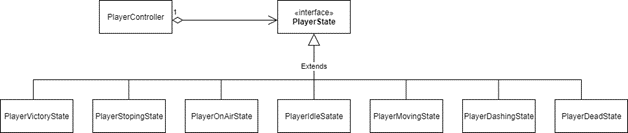
\includegraphics[scale=1]{Memoria/Aspectos_relevantes/Arquitectura_Player/Estados_Player}
\caption{Diagrama de transición entre estados de PlayerController}
\end{figure}

Adicionalmente la interfaz PlayerState añade los métodos EnterPlayerState y ExitPlayerState donde los hijos implementan las instrucciones que es necesario hacer para que al entrar y salir del estado el Player se mantenga consistente.

Las instrucciones que se llevan a cabo cada vez que se cambia de estado son las siguientes:

\begin{figure}[h]
\centering
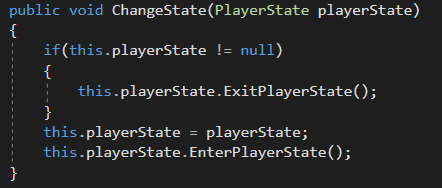
\includegraphics[scale=1]{Memoria/Aspectos_relevantes/Arquitectura_Player/Codigo_cambio_estado}
\caption{Diagrama de transición entre estados de PlayerController}
\end{figure}

\subsection{Interfaz PlayerMechanic}
Las mecánicas de salto, el acelerón y la mecánica de tiempo bala que puede realizar el Player han sido implementadas en tres clases que heredan de la interfaz PlayerMechanic. Esta interfaz incluye tres métodos: ManageInput para encargarse de comprobar si están pulsando los botones necesarios para llevar a cabo la mecánica, ManageFlags para gestionar los booleanos utilizados para saber si se va a llevar a cabo la mecánica o no, y ExecuteMechanic para ejecutar la mecánica (si se cumplen las condiciones necesarias para llevarla a cabo).

\begin{figure}[h]
\centering
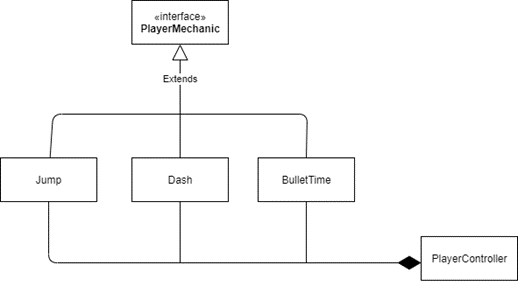
\includegraphics[scale=1]{Memoria/Aspectos_relevantes/Arquitectura_Player/PlayerMechanics}
\caption{Diagrama UML de la implementación de las mecánicas en PlayerController mediante composición}
\end{figure}

\section{Sistema de colisiones \cite{ContinuousCollision}\cite{UnderstandingConstraints}}
El objeto Player es un objeto con un Rigidbody2D kinemático. Para que dos objetos choquen al colisionar de manera ideal en el entorno de Unity es necesario que los objetos que colisionan tengan los componentes Collider y Rigidbody. Es necesario que el atributo BodyType del Rigidbody sea de tipo Dinamic. Cuando el Rigidbody es dinámico, Unity simula físicas sobre ese objeto. Como en el juego se va a trabajar con un sistema de físicas propio, el Rigidbody de los objetos con el componente KinematicObject no puede ser dinámico sino kinemático (BodyType = Kinematic). El problema de los RigidBody kinemáticos reside en que cuando se colisiona con objetos no se simula el choque entre ellos. Esto provoca que el Player atraviese el suelo y las paredes a pesar de entrar en contacto con ellos.

\subsection{Solución propuesta para el sistema de colisiones}
Ha sido necesario desarrollar un algoritmo para saber en cada loop del FixedUpdate si un KinematicObject esta colisionando con un muro. Para ello se hace uso de su velocidad para calcular la próxima posición del KinematicObject.\\
Con la próxima posición del juego calculada se comprueba si en esa posición hay algún muro, y en caso de ser así, se modifica la velocidad para que no colisione con el muro.

Un ejemplo de la modificación realizada sería:\\
El Player va a una velocidad de (3,-9.8), y debajo suyo hay un muro. La colisión se detectará y será necesario eliminar el movimiento hacia abajo del Player. Para saber que el movimiento del jugador debe se detenido hacia la abajo y no en el resto de direcciones se utiliza el vector normal del lado del muro más cercano al Player.

Después de detectar que dirección del movimiento se debe frenar para no colisionar con las paredes, se reducirá la velocidad en esa dirección.\\
En el ejemplo puesto anteriormente se va a detectar que se debe reducir la velocidad en el eje de las Y, quedando la velocidad en (3, 0).

En el anexo C se profundiza más en el tema.

\section{Sistema de gestión de las modificaciones gravitatorias}
Los objetos kinemáticos pueden recibir modificaciones gravitatorias que alteren su velocidad. De esta labor se encarga la clase KinematicObjectGravityManager.\\
Esta clase tiene una lista con todas las alteraciones gravitatorias que se aplicarán en ese loop del FixedUpdate. En cada loop del FixedUpdate se aplicarán al KinematicObject asociado a esa instancia de KinematicObjectGravityManager, y se vaciará la lista.

Se explicasu funcionamiento en profundidad en el anexo C.

\subsection{Obstáculos superdensos}
Los obstáculos superdensos son GameObject con una región de influencia (delimitada por un Collider2D). Mientras un KinematicObject esté dentro de la región de influencia su gravedad se verá modificada.

\begin{figure}[h]
\centering
\includegraphics[scale=1]{Memoria/Aspectos_relevantes/Modificaciones_gravitatorias/GameObject_obstáculo_superdenso}
\caption{Estructura del GameObject asociado al obstáculo superdenso (Dense Obstacle)}
\end{figure}

La fuerza de la gravedad con la que el objeto kinemático es atraído hacia el obstáculo depende de la distancia a la que se encuentre del obstáculo (mientras permanezca dentro de la región de influencia) siguiendo una función lineal $y=-m*x+n.$

La Y corresponderá con la modificación ejercida por el obstáculo, la pendiente corresponderá con la influencia que ejerce el obstáculo (InfluenceZone.gravityInfluence), X será la distancia al obstáculo y la ordenada en el origen corresponderá con la influencia máxima ejercible por el obstáculo (InfluenceZone.maxInfluence).

\begin{figure}[h]
\centering
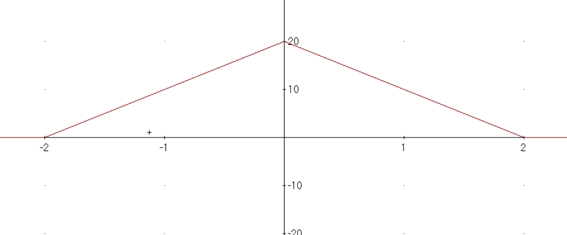
\includegraphics[scale=0.6]{Memoria/Aspectos_relevantes/Modificaciones_gravitatorias/Grafica_obstaculo_superdenso}
\caption{Gráfica que representa la influencia gravitatoria para una influencia máxima de 20, una influencia de 10 y un radio de región de influencia de 2 ($y = -10|X| + 20$)}
\end{figure}
\clearpage

Mientras se esté dentro de la región de influencia de un obstáculo superdenso se calculará el Vector2 que represente la influencia que ejerce sobre el KinematicObject y se añadirá a la lista de alteraciones de gravedad de la clase KinematicObjectGravityManager mediante el método AddGravityAlteration(Vector2).

\subsection{Inversor de gravedad}
Los inversores de gravedad invierten la gravedad del KinematicObject permanentemente al entrar en contacto con ellos. Para representar este proceso, se ha seguido una estructura de clases muy similar al patrón de diseño Observador. Hay una clase sujeto GravityInverterManager encargada de invertir la gravedad de los KinematicObjects y una clase observador GravityInverter encargada de decirle al sujeto que KinematicObjects tienen que invertir sus gravedades.

Cuando un observador detecta que un KinematicObject entra en contacto con él, le manda este KinematicObject al sujeto que comprueba si el KinematicObject está dentro de su lista y si no lo está lo añade. Si lo esta es removido de la lista.

En cada FixedUpdate el GravityInverterManager invierte la gravedad de todos los KinematicObject de la lista.

\begin{figure}[h]
\centering
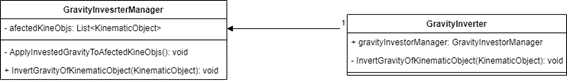
\includegraphics[scale=1]{Memoria/Aspectos_relevantes/Modificaciones_gravitatorias/Inversor_gravedad_UML}
\caption{Diagrama UML de la estructura del inversor de gravedad}
\end{figure}

\begin{figure}[h]
\centering
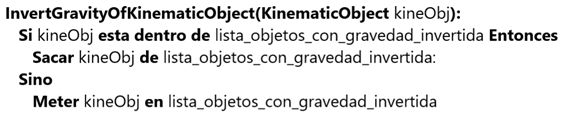
\includegraphics[scale=1]{Memoria/Aspectos_relevantes/Modificaciones_gravitatorias/Pseudocodigo_inversor_gravedad}
\caption{Pseudocódigo del método llamado cada vez que un KinematicObject entra en contacto con un inversor de gravedad}
\end{figure}

\begin{figure}[h]
\centering
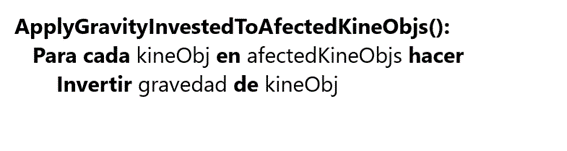
\includegraphics[scale=1]{Memoria/Aspectos_relevantes/Modificaciones_gravitatorias/Pseudocodigo_inverion_gravedad}
\caption{Pseudocódigo del proceso de inversión de gravedad de los KinematicObject en el FixedUpdate}
\end{figure}

Se ha creado un prefab que implementa el sistema de inversión gravitatoria llamado GravityInverterSystem que implementa todos los elementos necesarios para tener un sistema de inversión gravitatoria funcional.

\begin{figure}[h]
\centering
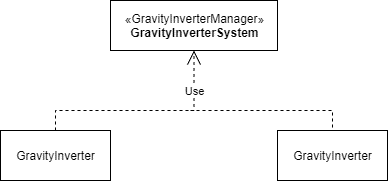
\includegraphics[scale=1]{Memoria/Aspectos_relevantes/Modificaciones_gravitatorias/GravityInverter_UML}
\caption{Estructura del prefab GravityInverterSystem}
\end{figure}

\section{Implementación de los obstáculos}
Los obstáculos son objetos que matan al Player al entrar en contacto con ellos. Hay tres tipos distintos de obstáculos: los obstáculos estáticos, los obstáculos que siguen una rutina y los obstáculos móviles.

\subsection{Obstáculos estáticos}
Los obstáculos estáticos son obstáculos que ocupan siempre la misma posición.

\begin{figure}[h]
\centering
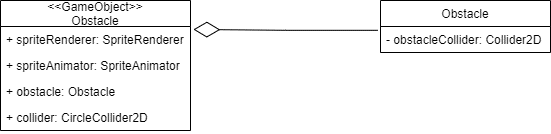
\includegraphics[scale=1]{Memoria/Aspectos_relevantes/Obstáculos/GameObject_obstaculo_estatico}
\caption{Estructura del GameObject asociado al obstáculo estático}
\end{figure}

Cuando una instancia de PlayerController entra en contacto con el Collider2D del obstáculo (Obstacle.obstacleCollider) se activa el evento PlayerObstacleCollision, que simplemente mata al Player y lo hace reaparecer en el punto de reaparición.

La estructura del obstáculo estático y la clase Obstacle son sencillas pero importantes, pues de ellas partirán el resto de obstáculos.

\begin{figure}[h]
\centering
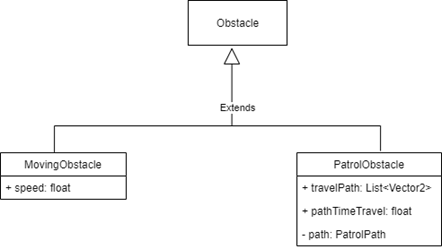
\includegraphics[scale=1]{Memoria/Aspectos_relevantes/Obstáculos/Herencia_obstaculos}
\caption{Jerarquía de herencia en la que el obstáculo móvil y el obstáculo que sigue una rutina heredan del obstáculo estático.}
\end{figure}

\subsection{Obstáculos que siguen una rutina}
Son obstáculos que viajan a través de una serie de puntos a una velocidad constante en un intervalo de tiempo marcado de manera repetitiva hasta el final de la ejecución de la escena. El punto de inicio y fin de la rutina coinciden. 

Realmente el obstáculo que sigue una rutina (PatrolObstacle) no calcula a donde tiene que moverse, sino que delega esta labor a la clase PatrolPath y mueve su posición a donde le indica el PatrolPath.

\begin{figure}[h]
\centering
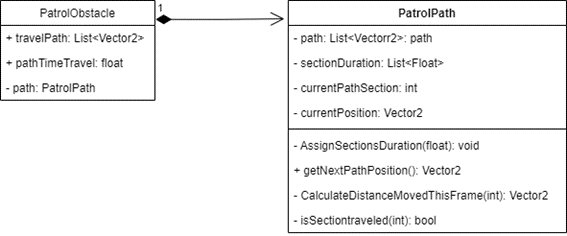
\includegraphics[scale=1]{Memoria/Aspectos_relevantes/Obstáculos/PatrolPath_UML}
\caption{Diagrama UML de la clase PatrolObstacle}
\end{figure}

PatrolPath recibe en el constructor la rutina que va a seguir el PatrolObstacle y el tiempo que tardará en recorrerla. PatrolPath calcula el tiempo que le llevará recorrer cada sección. Siendo que se tarda en hacer toda la rutina \textit{t} segundos, cada sección se tardará en recorrer $\dfrac{dy*d}{t}$

Siendo \textit{dy} la distancia euclidiana de la sección y \textit{d} la distancia total.

\begin{figure}[h]
\centering
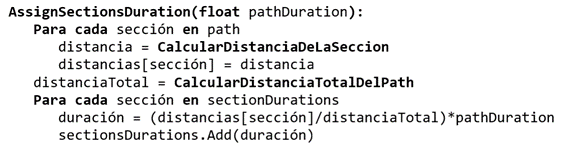
\includegraphics[scale=1]{Memoria/Aspectos_relevantes/Obstáculos/Pseudocodigo_asignar_duraciones}
\caption{Pseudocódigo de cálculo del tiempo que lleva recorrer cada sección}
\end{figure}

\clearpage
\begin{figure}[h]
\centering
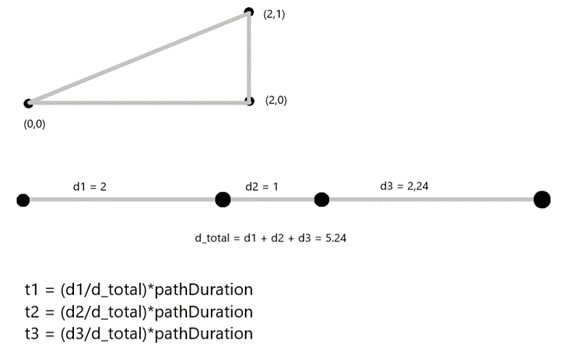
\includegraphics[scale=1]{Memoria/Aspectos_relevantes/Obstáculos/Diagrama_distancias_recorridas}
\caption{Cálculo del tiempo que se tarda en atravesar cada sección}
\end{figure}

PatrolPath sigue un diseño muy parecido al de un Iterador en el sentido de que el de la posición actual solo se puede obtener la siguiente y nada más.
La próxima posición del obstáculo que sigue una rutina (calculada en cada Update) se calcula sumando a la posición actual la distancia que se recorrerá cada frame (cada Time.deltaTime segundos).
La distancia que se recorre cada frame se puede obtener mediante la formula $\dfrac{(v1-v2)t}{ty}$

Siendo \textit{v1} el punto del que se parte, \textit{v2} el punto al que se quiere llegar, \textit{t} la fracción de espacio que se quiere recorrer (Time.deltaTime) en unidades de tiempo normalizado con\textit{ty} (el tiempo que se tarda en recorrer la sección) (en un frame se recorre un \textit{t/ty} sobre 1 de la distancia a recorrer).

\clearpage
\begin{figure}[h]
\centering
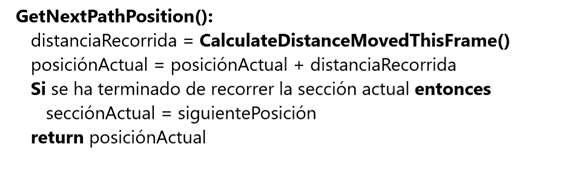
\includegraphics[scale=1]{Memoria/Aspectos_relevantes/Obstáculos/Pseudocodigo_siguiente_posicion}
\caption{Calcular la siguiente posición a la que debe moverse el obstáculo que sigue una rutina}
\end{figure}

\subsection{Obstáculos móviles}
Los obstáculos móviles son obstáculos que parten de un punto inicial y avanzan indefinidamente de izquierda a derecha a una velocidad establecida. La posición del obstáculo móvil en el frame actual se calcula añadiendo a la posición actual el vector dirección (Vector2.lef) por la velocidad establecida y por el tiempo entre frames (Time. fixedDeltaTime).

Esto se lleva a cabo mediante la instrucción ejecutada en cada FixedUpdate:

this.transform.position += (Vector3) Vector2.left * speed * Time.fixedDeltaTime;

\subsection{Clase ObstacleFabric}
Ante la necesidad de crear obstáculos móviles durante tiempo de ejecución se creó la clase ObstacleFabric. Esta clase es una aplicación del patrón de diseño Método Fabrica. ObstacleFabric tiene un método SpawnObject que devuelve una instancia del prefab establecido en la posición en la que se encuentra la fábrica.

De ObstacleFabric hereda una clase TriggerObstacleFabric que tiene asociada una clase PlayerTrigger. La clase PlayerTrigger es una clase que tiene asociado un Collider2D. PlayerTrigger tiene un atributo booleano isTrigger y mientras una instancia de PlayerController este en contacto con el collider de PlayerTrigger isTrigger será true y el resto del tiempo a false.

Cuando el Player entre en la zona de activación de PlayerTrigger (delimitada por el collider), TriggerObstacleFabric creará una instancia del prefab.

\begin{figure}[h]
\centering
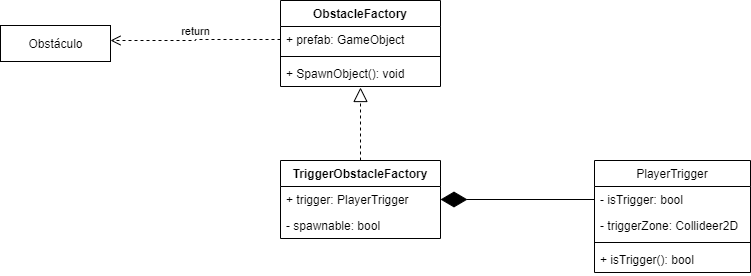
\includegraphics[scale=0.8]{Memoria/Aspectos_relevantes/Obstáculos/ObstacleFabric_UML}
\caption{Diagrama UML de la estructura de las fábricas de obstáculos}
\end{figure}

La intención de ObstacleFabric era que solo pudiese instanciar obstáculos, pero al elegir el obstáculo que se desea instanciar mediante la elección de un prefab lo que se pasa a instanciar es un GameObject y no un obstáculo, haciendo que aunque la fábrica se utilice exclusivamente para instanciar obstáculos, realmente se puede instanciar cualquier GameObject.

\subsection{Clase ObstacleDestroyer}
Los obstáculos móviles tienen una vida útil muy corta pues solo son necesarios desde que aparecen hasta que han atravesado toda la pantalla. Sin embargo cuando han perdido utilidad siguen desplazándose hacia la derecha consumiendo recursos de manera similar a como lo haría un proceso zombie. Para evitar esto se ha creado una clase ObstacleDetroyer que tiene asociado un Collider2D. Cuando los obstáculos entran en contacto con el collider del ObstacleDestroyer, el obstáculo se destruye liberando los recursos ocupados en él.

\section{Implementcación de los portales}
Los portales son GameObject organizados por parejas que permiten convertir la posición de un KinematicObject que entra a un portal en la posición del portal parejo al portal de aquel por el que se ha entrado (simulando la teletransportación entre portales).\\
Es una clase muy sencilla. La única complejidad reside en desactivar los portales durante el proceso de teletransportación para evitar que el KinematicObject se quede enganchado teletransportándose infinitamente de un portal a otro; y reactivarlos al salir del portal.

\begin{figure}[h]
\centering
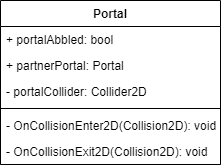
\includegraphics[scale=1]{Memoria/Aspectos_relevantes/Portales/Portales_UML}
\caption{Diagrama UML de la clase Portal}
\end{figure}

Como se ha mencionado anteriormente, los Portales se organizan en parejas. Se ha creado un prefab PortalCouple que es un GameObject con un par de portales asociados entre sí.

\begin{figure}[h]
\centering
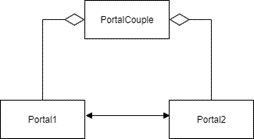
\includegraphics[scale=1]{Memoria/Aspectos_relevantes/Portales/Couple_portals}
\caption{Estructura de relaciones del GameObject PortalCouple}
\end{figure}

\section{Creadores de impulso}

Los creadores de impulso son objetos que aplican una variación en la velocidad que llevan a los objetos kinemáticos que entran en contacto con ellos. Hay tres tipos de creadores de impulso: la plataforma de salto, la partícula de impulso y el amplificador de impulso.
Para los creadores de impulso se ha decidido aplicar el patrón de diseño Puente.
\clearpage

\begin{figure}[h]
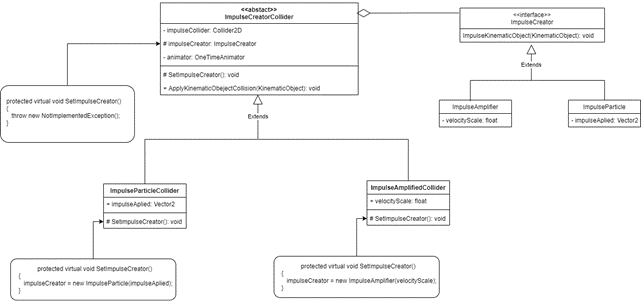
\includegraphics[scale=0.8]{Memoria/Aspectos_relevantes/Creadores_impulso/Creadores_impulso_UML}
\caption{Estructura de relaciones del GameObject PortalCouple}
\end{figure}

No se he decidido aplicar el patrón Puente porque el funcionamiento de los creadores de impulso valla a cambiar en tiempo de ejecución (que no lo hace), sino para reforzar la separación ente las clases encargadas de detectar las colisiones y las clases encargadas de aplicar el impulso evitando un vínculo permanente entre estas dos jerarquías de clases que haga más engorroso el proceso de adición o modificación de clases en una de las dos jerarquías establecidas.

\subsection{Sistema de gestión de las colisiones con los creadores de impulso}
Las colisiones de los creadores de impulso con los KinematicObject se han implementado siguiendo el mismo modelo que la colisión con los “Wall” (paredes y muros). La clase KinematicObjectCollisionManager llama al método BoxCastAll en la posición en la que se va a encontrar el KinematicObject en el siguiente frame. Si va a haber colisión con un creador de impulso se invoca al método ApplyKinematicObjectCollision del ImpulseCreatorCollider que delega la labor de aplicar el impulso a la instancia de ImpulseCreator que tiene asociada.\\
Explicado a grandes rasgos KinematicObjectCollisionManager avisa a ImpulseCreatorCollider de que se va a producir una colisión y este ordena a ImpulseCreator que aplique el impulso correspondiente al KinematicObject asociado al KinematicObjectCollisionManager.

\subsection{Tipos de creadores de impulso}
\subsubsection{Partícula de impulso}
Objeto que aplica un impulso en la dirección marcada por un Vector2 (ImpulseParticle.impulseAplied).

\begin{figure}[h]
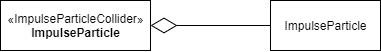
\includegraphics[scale=0.8]{Memoria/Aspectos_relevantes/Creadores_impulso/Particula_impulso}
\caption{Estructura del prefab asociado a la partícula de impulso}
\end{figure}

\subsubsection{Plataforma de salto}
Objeto similar a la partícula de impulso pero con la excepción de que el impulso aplicado solo puede ser en el eje vertical (ImpulseParticle.impulseAplied.X será siempre 0).

\begin{figure}[h]
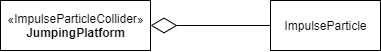
\includegraphics[scale=0.8]{Memoria/Aspectos_relevantes/Creadores_impulso/Plataforma_salto}
\caption{Estructura del prefab asociado a la plataforma de impulso}
\end{figure}

\subsubsection{Amplificador de impulso}
Objeto similar a la partícula de impulso, solo que en vez de añadir un impulso escala la velocidad que lleva el objeto kinemático con el que colisionag. La velocidad se escala ImpulseAmplifier.velocityScale veces.

\begin{figure}[h]
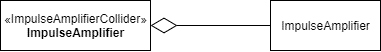
\includegraphics[scale=0.8]{Memoria/Aspectos_relevantes/Creadores_impulso/Amplificador_impulso}
\caption{Estructura del prefab asociado al amplificador de impulso}
\end{figure}

\section{Animación de los sprites}
Salvo para el Player, que se ha utilizado un animator de Unity, para el resto de objetos que requerían de un proceso de animación ha sido necesaria la creación de clases encargadas de la animación de estos objetos.\\

\begin{figure}[h]
Las clases encargadas de la animación son SpriteAnimator y OneTimeAnimator.

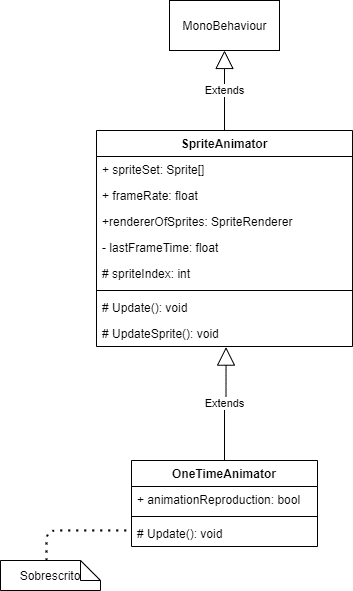
\includegraphics[scale=0.8]{Memoria/Aspectos_relevantes/Animadores/Herencia_animators}
\caption{Estructura de herencia de los animadores de sprites}
\end{figure}

Ambos animadores de sprites se encargan de reproducir una animación marcada por un vector de Sprite dado (SpriteAnimator.spriteSet). La diferencia entre las dos clases es que SpriteAnimator reproduce la animación en bucle indefinidamente (si llega al último Sprite del vector, el siguiente será el primero del vector), mientras que OneTimeAnimator reproducirá la animación una sola vez (cuando la variable OneTimeAnimator. animationReproduction sea true).

\subsection{UpdateSprite()}
El método UpdateSprite es el encargado de generar el efecto de reproducción de una animación mediante su llamada en cada Update. UpdateSprite cambia el Sprite a renderizar por el SpriteRenderer del GameObject cada $\frac{1}{SpriteAnimator.frameRate}$ segundos.

 
Esta división surge de que SpriteAnimator.frameRate lleva la cuenta de cuantos Sprites se tienen que reproducir en un segundo, con lo que cada $\frac{1}{SpriteAnimator.frameRate}$ se actualizará el Sprite a renderizar.

Para saber si hay que pasar a renderizar el siguiente Sprite se consulta la variable SpriteAnimator.lastFrameTime, que guarda el momento de tiempo en el que se actualizó por última vez el Sprite del SpriteRenderer. Cuando la diferencia entre Time.time (variable float que cronometra cuanto tiempo de ejecución lleva el programa) y SpriteAnimator.lastFrameTime sea mayor que $\frac{1}{SpriteAnimator.frameRate}$ (el tiempo transcurrido entre actualizaciones de Sprites) se actualizará el Sprite a renderizar y se recalculará SpriteAnimator.lastFrameTime.

\begin{figure}[h]
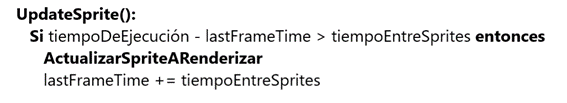
\includegraphics[scale=1]{Memoria/Aspectos_relevantes/Animadores/Pseudocodigo_UpdateSprite}
\caption{Pseudocódigo de UpdateSprite}
\end{figure}

\section{Clase GameController y estado de juego estable}
Durante la ejecución de las escenas hay elementos que se requiere que estén en una posición inicial y que se pueda volver a ella cuando se requiera (concretamente cuando el Player muera y se tenga que volver al estado inicial de la escena).\\
Los objetos que gestiona el GameController puede ser cualquier GameObject, pero no todos necesitarán ser reiniciados, pues tendrán un estado estable durante toda la ejecución de la escena. Por ejemplo, los obstáculos móviles se desplazan horizontal y pueden incluso ser destruidos, pero cuando el Player muera el obstáculo móvil tiene que volver a la posición inicial en la que se encontraba al cargar la escena. De esta labor se encargará el GameController. Sin embargo, el obstáculo inmóvil se mantiene siempre estático en la misma posición y no puede ser destruido, con lo que el GameController no tiene que preocuparse por devolverlo a un estado estable, pues es el único estado en el que puede estar.

\begin{figure}[h]
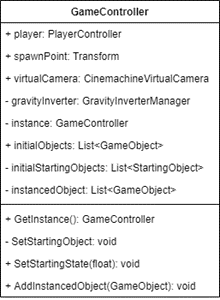
\includegraphics[scale=1]{Memoria/Aspectos_relevantes/GameController/GameController}
\caption{Diseño de la clase GameController}
\end{figure}

GameController está implementado de manera que simule el patrón de diseño Singleton, en la medida en la que Unity lo permite, llamándose en el método Awake al método GetInstance() para asegurarse de que siempre se trabaja siempre sobre el mismo GameController, a pesar de que haya varias instancias de él.

\subsection{Funcionamiento del estado estable}
GameObject tiene tres atributos lista: initialObjects, initialStartingObjects e instancedObjects. De estas tres listas la única pública es initialObjects. La intención de esta lista es que se añada en el editor de Unity todos los elementos cuyo estado se desea que sean devueltos a un estado estable.\\
Cuando se llama al método Awake el contenido de initialObjects se vuelca en initialStartingObjects. InitialStartingObjects no es una lista de GameObject sino una lista de StartingObject. La clase StartingObject es una clase que contiene dos atributos: el GameObject que se desea poder devolver a un estado estable y un atributo Transform con la información necesaria para devolver el GameObject a la posición inicial.\\
Por último la lista instancedObject contiene los objetos que hay que se han devuelto al estado estable.

Estas tres listas pueden parecer redundantes, pero no lo son. Es cierto que entre intialObjects e initialStartingObjects no hay mucha diferencia, pero al ser pública la lista initialObjects se ha preferido crear una lista con un nivel de encapsulamiento privado y que haya tratado los elementos de initialObjects para adaptarse a la aplicación del estado estable. Los elementos de StartingObjects en realidad van a hacer la labor de prototipo. Esto se refiere a que los elementos de initialStartingObjects no van a aparecer en la escena, sino que van a ser utilizados para clonar GameObjects en el estado inicial deseado para que parezca que todos los elementos vuelven a su estado inicial, cuando en realidad están siendo destruidos e instanciados objetos iguales a los eliminados (esto es lo que hace el método SetStartingState).

Los elementos que tiene la lista instancedObjects son todos los GameObject que se van a destruir cuando se llame al método SetStartingState. InstancedObjects por supuesto tendrá todos los objetos clonados de initialStartingObjects, pero también contiene GameObjects que pueden ser creados en tiempo de ejecución pero que al volver el juego a un estado inicial tienen que ser destruidos (como por ejemplo los obstáculos móviles que instancian las fábricas de obstáculos).

\begin{figure}[h]
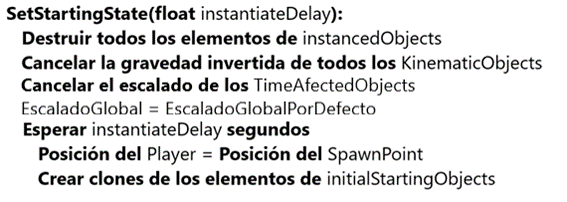
\includegraphics[scale=1]{Memoria/Aspectos_relevantes/GameController/Pseudocodigo_starting_objects}
\caption{Pseudocódigo que refleja todas las operaciones que hay que realizar para establecer un estado de juego inicial estable}
\end{figure}

\subsection{Clase PlatformerModel}
La clase PlatformerModel es una clase estática con atributos estáticos y sin métodos. La intención de esta clase es ofrecer acceso a una serie de objetos que pueden ser necesitados por cualquier clase en la escena. La única clase que debería asignar valores a PlatformerModel es GameObject, que lo hará exclusivamente en la llamada al método Awake y realizará la asignación una sola vez y no modificará en ningún momento más durante la ejecución los valores de los atributos de PlatformerModel. Los objetos que se podrán consultar mediante PlatformerModel son:
\begin{itemize}
\item
La CinemachineVirtualCamera que utiliza la escena (PlatformerModel.virtualCamera).
\item
El PlayerController asignado al avatar jugable (PlatformerModel.player).
\item
El objeto de tipo Transform asociado al punto de reaparición e inicio de escena del Player (PlatformerModel.spawnPoint).
\item
El GameController de la escena (PlatformerModel.gameController).
\item
El GravityInverterManager asociado a la escena \\ (PlatformerModel.gravityInverterManager).
\end{itemize}
Esta clase es muy útil para asegurar que todas las clases trabajan sobre los mismos objetos , sobre todo los eventos, pues puede resultar inadecuado hacer una cadena de mensajes para que los eventos tengan referencias a todos los objetos que puedan necesitar para realizar la operaciones que tienen que llevar a cabo.

\subsection{Clase Simulation}
La clase Simulation esta explicada más detalladamente en la sección de Trabajos relacionados. Pero a grandes rasgos la clase Simulation es una clase estática con una estructura de datos similar a una cola que alberga eventos y un método Tick. Ese método lo que hace es ir avanzando eventos en la cola y ejecutándolos hasta que la cola este vacía o hasta que se encuentre un evento que debe ser ejecutado en un momento de la ejecución posterior al momento en el que se encuentra el programa.

\clearpage
\begin{figure}[h]
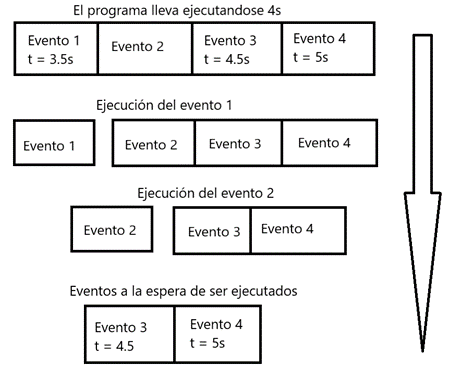
\includegraphics[scale=1]{Memoria/Aspectos_relevantes/GameController/Flujo_simulation}
\caption{Diagrama que representa un ejemplo de las operaciones llevadas a cabo en la llamada al método Tick}
\end{figure}

La clase GameController llama al método Tick de Simulation en cada llamada al Update.

\section{Mecánicas de tiempo bala}
Se han implementado una serie de mecánicas encargadas de escalar la velocidad a la que pasa el tiempo y como esto afecta a los objetos en la escena. Hay dos mecánicas de tiempo bala: escalar el tiempo a nivel global y escalar el tiempo de los objetos dentro de una zona. De los dos escalados de tiempo se encarga la clase TimeManager.

\clearpage
\begin{figure}[h]
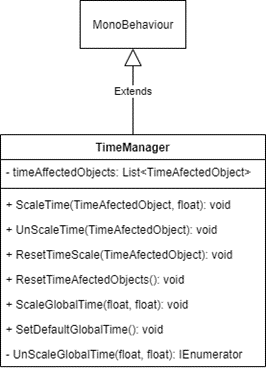
\includegraphics[scale=1]{Memoria/Aspectos_relevantes/Tiempo_bala/TimeManager_UML}
\caption{Diagrama UML de la clase TimeManager}
\end{figure}

\subsection{Escalado de tiempo global}
Es escalado de tiempo global es muy sencillo, pues Unity ya ofrece una herramienta que modifica el tiempo de todos los objetos. Se trata de la variable Time.scaleTime y todos los objetos relacionados con Unity se ven afectados por esta variable, incluidos los eventos (no los de la clase Simulation sino los propios de Unity).

A grandes rasgos Time.timeScale funciona multiplicando su valor por el “tiempo que tardará en llevarse a cabo la acción”. Siendo que si se tarda en ir de un punto ‘A’ a uno ‘B’ en X tiempo, se tardará en verdad X*Time.timeScale unidades de tiempo.

Del escalado del tiempo para todos los objetos se encargan las funciones TimeManager.ScaleGlobalTime, TimeManager.UnScaleGlobalTime y TimeManager.SetDefaultGlobalTime.

El escalado de tiempo global se aplica en la mecánica de tiempo bala del Player, escalando el tiempo y desescalandolo al los X segundos; y se aplica también en el estado estable del GameController (GameController.SetStartingState()).

\subsection{Zonas de escalado de tiempo}
Las zonas de tiempo escalado son objetos con un Collider2D. Cuando entre un TimeAfectedObject en el Collider2D, la zona de tiempo escalado escalará su tiempo hasta que salga de él.

\begin{figure}[h]
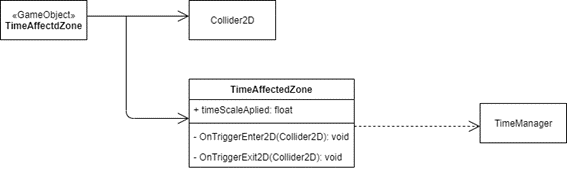
\includegraphics[scale=1]{Memoria/Aspectos_relevantes/Tiempo_bala/GameObject_zona_tiempo_escalado}
\caption{Estructura del GameObject asociado a las zonas de tiempo escalado}
\end{figure}

TimeAfectedObject es una clase abstracta de la que heredan los objetos que van a ser afectadas por las zonas de escalado de tiempo. TimeAfectedObject tiene el método abstracto Move, que es el que implementarán las clases con la intención de modificar el movimiento del objeto para adecuarse a la escala de tiempo que le ha sido aplicada.

\clearpage
\begin{figure}[h]
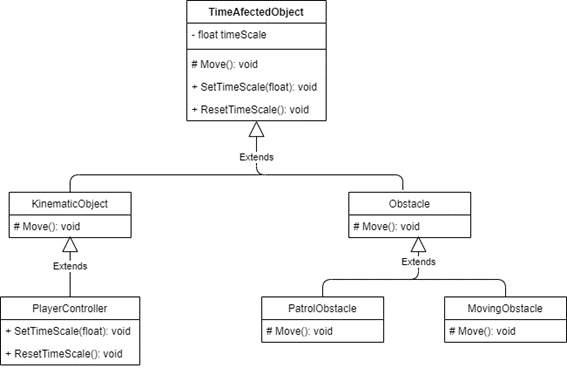
\includegraphics[scale=1]{Memoria/Aspectos_relevantes/Tiempo_bala/Herencia_TimeAffectedObject}
\caption{Estructura de herencia de TimeAfectedObject}
\end{figure}

Las zonas de escalado de tiempo imponen su escalado de tiempo a través de la clase TimeManager. Esto se debe a que TimeManager asume la responsabilidad de resetear el escalado de tiempo de todos los TimeAfectedObject. Esta necesidad surge de asegurar que en el estado de juego estable del GameController no haya TimeAfectedObject con el tiempo escalado. Es por ello que TimeManager tiene una lista de TimeAfectedObject en la que estarán todos los TimeAfectedObject cuyo tiempo haya sido escalado.

\begin{figure}[h]
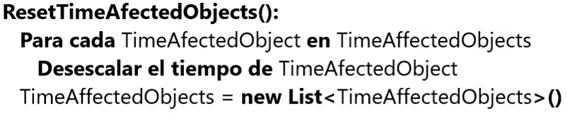
\includegraphics[scale=1]{Memoria/Aspectos_relevantes/Tiempo_bala/Pseudocodigo_TimeAffectedObject}
\caption{Pseudocódigo del método llamado para resetear los TimeAfectedObject}
\end{figure}

\section{Menús de los juegos}
Se ha desarrollado un sistema de menús de juego y transiciones entre escenas.

\begin{figure}[h]
\includegraphics[scale=1]{Memoria/Aspectos_relevantes/Menus/Transición_entre_menus}
\caption{Diagrama de viaje entre los distintos menús y escenas}
\end{figure}

La escena de la que se parte es la escena de selección de nivel. De esta escena se puede cerrar la aplicación (botón “Exit”), pasar a la escena de menú de opciones y jugar el nivel que se escoja.
En el nivel jugable se puede abrir un menú de pausa que detiene la ejecución del nivel jugable hasta que se cierre el menú de pausa.
Lo que se puede hacer en el menú de pausa y en el menú de opciones es básicamente lo mismo. Sin embargo, son objetos distintos (uno es un canvas y otro es una escena) con navegación a escenas distintas. Adicionalmente, el menú de pausa tiene la tarea añadida de parar la ejecución de la escena. Es por esto que se han tratado y desarrollado como elementos distintos.

\subsection{Menú de pausa}
El menú de pausa es un objeto con dos elementos fundamentales: la clase OptionsCanvasManager y un objeto hijo del menú de pausa que es un Panel.

\clearpage
\begin{figure}[h]
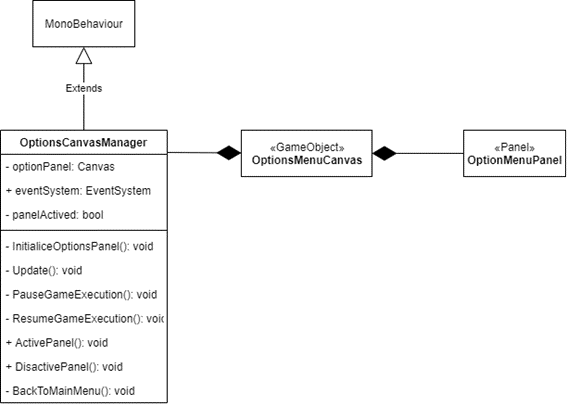
\includegraphics[scale=1]{Memoria/Aspectos_relevantes/Menus/GameObject_menu_pausa}
\caption{Diagrama de la estructura de GameObject asociado al menú de pausa}
\end{figure}

OptionsCanvasManager se encarga de abrir y cerrar el menú al pulsar el botón correspondiente y pausar y retomar la ejecución de la escena respetivamente (OptionsCanvasManager.PauseGameExecution y OptionsCanvasManager.ResumeGameExecution).

Lo que se hace en verdad al abrir y cerrar el menú de pausa es activar y desactivar el Panel (que muestra la interfaz del menú de pausa) y el EventSystem (se explicará en el siguiente apartado).

\begin{figure}[h]
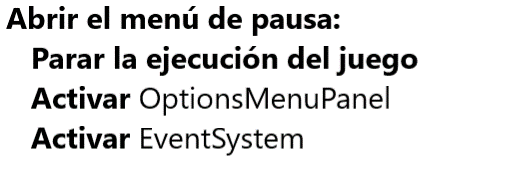
\includegraphics[scale=1]{Memoria/Aspectos_relevantes/Menus/Pseudocodigo_abrir_menu_pausa}
\caption{Pseudocódigo de las operaciones llevadas a cabo al abrir el menú de pausa}
\end{figure}

\begin{figure}[h]
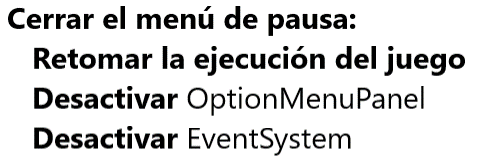
\includegraphics[scale=1]{Memoria/Aspectos_relevantes/Menus/Pseudocodigo_cerrar_menu_pausa}
\caption{Pseudocódigo de la operaciones llevadas a cabo al cerrar el menú de pausa}
\end{figure}

\subsection{Método de selección de elementos UI}
Para navegar entre los elementos del menú de utiliza un objeto de la clase EventSystem. Este objeto se encarga de manejar eventos de Unity (que no tienen nada que ver con los eventos de Simulation). Este objeto se utiliza para captar los botones de navegación pulsados y navegar al elemento UI correspondiente. Es por esto que al abrir y cerrar el menú de opciones también se activa y desactiva el EventSystem. Si no se desactiva el EventSystem los elementos del menú de opciones variarán en función de los botones pulsado a pesar de estar cerrado (por ejemplo modificando el volumen del juego sin abrir el menú de opciones). 

\subsection{Patrón de colores utilizados}
El patrón de colores utilizado para los elementos UI es el siguiente:

\clearpage
\begin{figure}[h]
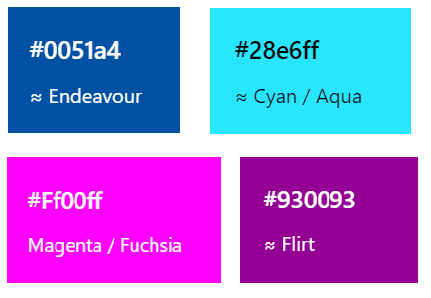
\includegraphics[scale=1]{Memoria/Aspectos_relevantes/Menus/Patron_colores}
\caption{Patrón de colores utilizado para la UI}
\end{figure}

\section{Sistema de modificación de volumen persistente}
En las opciones hay dos opciones: una que permite variar el volumen general del juego y otra que permite variar el volumen de las canciones que suenan. La idea es que cambiar el volumen haga este cambio persistente, manteniéndose entre escenas y ejecuciones del programa. Para ello han sido necesarias dos clases: VolumeManager y AudioSourceVolumeManager.

VolumeManager es una clase estática encargada de consultar y modificar el valor persistente de ambos tipos volumen. Este valor corresponde con el valor del volumen del juego que se encargará de leer y modificar VolumeManager y de compartirlo con las instancias de AudioSourceVolumeManager cuando lo requieran. Esto se hace mediante la clase PlayerPrefs, clase que ofrece Unity para guardar el valor de variables entre ejecuciones. Esto también se podría haber hecho guardando en un fichero los valores que se quiera que sean persistentes (que es lo que hace la clase PlayerPrefs al final), pero siendo que solo se desea almacenar el valor de variables se ha optado por la solución más simple. Si se hubiese querido se habría podido utilizar un fichero, pero hay que guardarlo en la ruta ofrecida por la variable Application.persistentDatatPath si se quiere que al exportar la aplicación se guarde y consulte correctamente el fichero.

La clase AudioSourceVolumeManager actúa como envoltorio del objeto AudioSource de Unity (el que se usa para reproducir audios). El volumen del AudioSource no se modifica explícitamente, sino que AudioSourceVolumeManager consulta el valor general del volumen en AudioSourceManager y se lo asigna al AudioSource del que tiene referencia. AudioSourceVolumeManager tiene una clase hija que es AudioSourceMusicVolumeManager, que modifica el volumen del AudioSource en función del volumen de la música además del volumen general.

\begin{figure}[h]
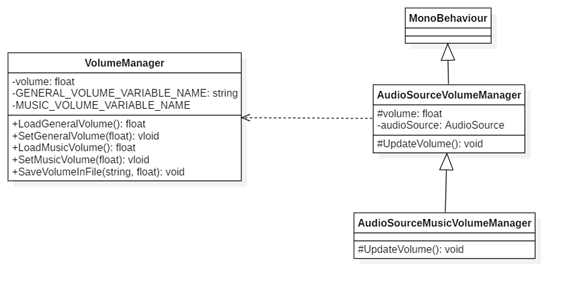
\includegraphics[scale=1]{Memoria/Aspectos_relevantes/Volumen_persistente/VolumeManager_UML}
\caption{Diagrama UML que representa la relación entre VolumeManager y AudioSourceVolumeManager}
\end{figure}

\subsection{Escenas que comparten canción}
Las escenas GameMenu y OptionsScene comparten canción, de manera que aunque se cambien entre estas dos escenas la canción que suena no dejará de reproducirse. En verdad sí que lo hará, pero lo que sucede es que al viajar entre estas escenas se guardará (en una variable estática) el segundo de la canción que se está reproduciendo y al entrar a la otra escena se reproducirá la canción pero continuando desde el punto en el que había dejado la canción la escena anterior. Cuando desde estas dos escena se viaje a una que no es esa, en vez de guardar el segundo de la canción en el que se está, se reseteará la variable donde se está guardando el segundo de la canción (poniéndolo a 0) y haciendo así que la próxima vez que se entre a estas escenas la canción se empiece a reproducir de cero.

\subsection{Clase VolumeSliderBar}
El volumen general se modifica en la clase VolumeSliderBar, que tiene asociado un elemento UI Slider. VolumeSliderBar consulta el valor del Slider y se lo asigna al volumen de VolumeManager. VolumeSliderBar es una clase abstracta con dos hijos: GeneralVolumeSliderBar para modificar el volumen general y MusicVolumeSliderBar para el volumen de las canciones que suenan.

\section{Desarrollo de la gestión de la cámara}
Se va a documentar en la memoria el proceso de desarrollo de la gestión de la cámara a la vez que se desarrolla, pues se considera un muy buen ejemplo de desarrollo de uno de los elementos de un videojuego y suficientemente representativo como para entender el proceso. Además va a resultar interesante, pues se va a razonar el funcionamiento de las cámaras y las decisiones que se han tomado para escoger un funcionamiento de la cámara y no otro.

La mayoría de la información obtenida para la toma de decisiones durante este proceso ha sido obtenida de la siguiente URL de la página de Gamasutra \cite{Gamasutra}:\\
 \url{https://www.gamasutra.com/blogs/ItayKeren/20150511/243083/Scroll_Back_The_Theory_and_Practice_of_Cameras_in_SideScrollers.php}.
 
Este enlace contiene otro enlace a una charla en la que se explican estos conceptos en video.

\subsection{Introducción al sistema gestor de cámaras}
La cámara va a ser el elemento encargado de mostrar por pantalla la región del espacio del nivel que se desea mostrar. El principal conflicto que afecta a la cámara es que en distintos momentos del juego se quiere mostrar espacios distintos del escenario. Por suerte este problema es más sencillo de lo que parece en un principio, pues la mayoría del rato las distintas regiones del espacio que se deseen mostrar estarán condicionados por un elemento principal que se mueven en el espacio (en el caso de este juego y la mayoría, ese elemento será el avatar que utilice el jugador). Ese problema tiene una solución relativamente sencilla y, sobre todo explorada por juego hechos en el pasado, que es hacer que la cámara siga a ese elemento principal.

En este videojuego, afortunadamente, el único elemento principal que hay que seguir es el jugador. En otros videojuegos esta tarea puede ser más compleja, ya sea debido a que cambia el objetivo principal (a un elemento que hay que perseguir o una pantalla que avanza con el tiempo por ejemplo) o que hay varios objetivos principales (como en un juego multijugador local o en una batalla contra un jefe, donde los objetivos principales son tanto el jugador, como el jefe).

Sin embargo, aunque solo haya un objetivo principal en el juego (el jugador), puede ser que en el haya objetivos secundarios que no merezcan que la cámara los siga específicamente a ellos, pero sí tenerlos en cuenta. En lo que se lleva de desarrollo hasta ahora hay dos objetivos secundarios que generan conflicto: los portales y los obstáculos. Estos objetivos secundarios son variados y generan conflictos distintos sobre la cámara. Se van a explicar a continuación.

\subsection{Conflictos con los portales}
Los portales son los elementos que más dudas me generan acerca de cómo afrontarlos. El problema de los portales es que trabajan en parejas. Al entrar por un portal, sales por el portal pareja de este, independientemente de si está en el rango de lo que permite ver la cámara. Con el sistema de gestión de cámaras que ofrece Plataformer Microgame (el usado hasta ahora) la cámara apunta exactamente al punto donde está el jugador. Esto para los portales resulta bastante conveniente, pues según el jugador atraviesa el portal la cámara sigue apuntando a la posición del jugador, dando visión instantáneamente del jugador dificultar la visión de lo que el jugador tiene ahora en su nuevo entorno. En términos de ofrecer visión al jugador es una solución bastante eficaz, pero adolece de un gran problema: el jugador ahora no sabe dónde está. El jugador ahora se haya desorientado. El jugador anteriormente tenía una referencia clara de donde se encontraba (básicamente se había a la derecha del punto de inicio), pero ahora no tiene ni idea de donde está ni adonde tiene que ir. La escena de prueba de los portales es una muy buena práctica para comprobar si el diseño de los portales desorienta o no.

\clearpage
\begin{figure}[h]
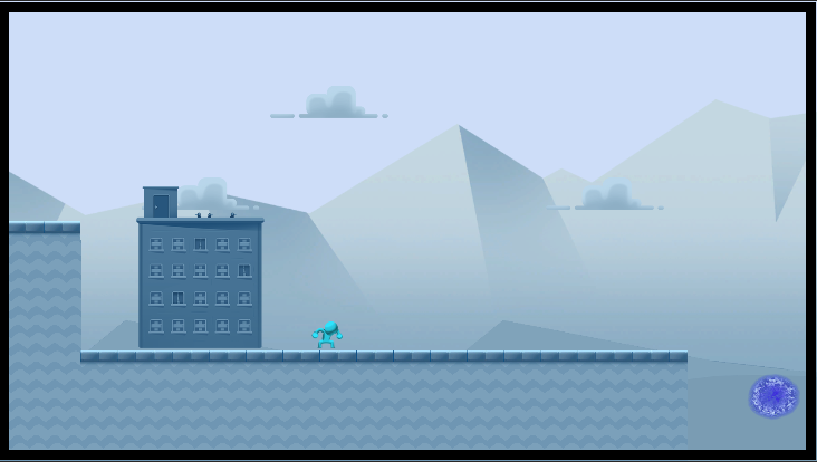
\includegraphics[scale=1]{Memoria/Aspectos_relevantes/Camaras/PruebaPortalScene}
\caption{Escena PruebaPortalScene}
\end{figure}

En la imagen se ha dibujado flecha en cada plataforma con el sentido que se espera que siga el jugador para llegar hasta la zona de victoria. En esta escena el jugador no solo no puede ver los dos portales que forman una pareja de portales y deducir por donde de donde ha venido, sino que además se está cambiando continuamente la dirección que se espera que tome el jugador tome. Un jugador probablemente no sea capaz de deducir que camino ha de tomar de manera intuitiva.

Una solución parcial a este problema podría ser al principio del nivel mostrar el nivel entero e ir haciendo Zoom-in hasta llegar al jugador y dejar la cámara en la posición que tendrá por defecto. Pero esto no es solo un parche improvisado al problema, sino que además en niveles grandes habrá demasiados elementos como para que ese recurso permita ver nada y mucho menos permitir al jugador deducir el camino que debe seguir.\\
Este problema no desaparece con este sistema de gestión de cámaras y se ha de tener en cuenta en el nuevo que se va a implementar.

El segundo problema que provocan los portales es una premonición del sistema que probablemente se acabe implementando. Se pretende que la cámara siga al jugador, no que apunte estrictamente a él. Con los portales surge el problema de que, al mover al jugador a una posición alejada del punto en el que se encontraba un frame antes, la cámara ahora se tiene que mover hasta ahí pudiendo hacer que en lo que llega la cámara ocurra algo que el jugador no haya visto. Reduces “innecesariamente” la información que el jugador puede obtener a través de la cámara. El problema de orientación del jugador que se soluciona con el sistema de cámara que se planea implementar se sustituye por este. Este problema se pude solucionar haciendo que no suceda nada en las cercanías de los portales pero a costa de limitar la creatividad y variedad que los portales ofrecen al salir de uno.

\subsection{Conflictos con los obstáculos}
Aquí el problema es solo uno: Puede ser que el tiempo de reacción ante la aparición de un obstáculo y el espacio que la cámara ofrece para que el jugador se dé cuenta de que está en riesgo de colisionar con un obstáculo sean demasiado pequeños. Este problema se va a separar en tres tipos de obstáculos y como estos manifiestan el problema recién explicado.

\textbf{Obstáculos estáticos:} Los obstáculos que probablemente menos conflictos generen son los obstáculos estáticos. En principio casi cualquier tamaño de cámara permitiría ver y reaccionar ante este obstáculo. Pero en el juego que se está desarrollando no se va a tener en todo claro que velocidad va a llevar el jugador y es posible que algún obstáculo se haga excesivamente difícil de esquivar solo por el un mal implementado sistema de gestión de la cámara. Unity adicionalmente puede provocar confusión al respecto, ya que las distancias pueden llegar a percibirse distintas en el editor que en la pantalla de juego.\\
Por ejemplo la escena PruebaPlayerScene en el editor da la impresión de haber suficiente distancia entre el jugador y el obstáculo, pero en la pantalla de juego se ve como la distancia es menor y dependiendo de la velocidad con la que el jugador llegue puede ser que el jugador no tenga suficiente tiempo de respuesta como para esquivar el obstáculo.

\begin{figure}[h]
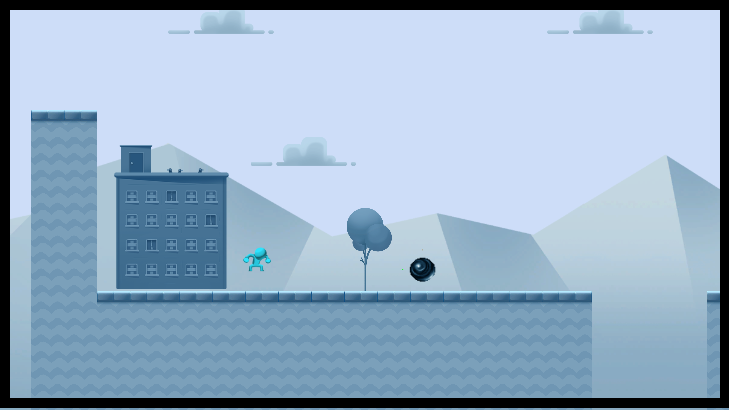
\includegraphics[scale=1]{Memoria/Aspectos_relevantes/Camaras/PruebaPlayerScene}
\caption{Escena PruebaPlayerScene}
\end{figure}

\clearpage
\begin{figure}[h]
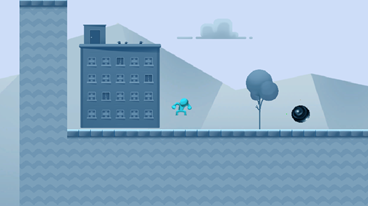
\includegraphics[scale=1]{Memoria/Aspectos_relevantes/Camaras/Camara_PruebaPlayerScene}
\caption{Visión de la escena PruebaPlayerScene desde la cámara.}
\end{figure}

\textbf{Obstáculos que siguen patrones:} Con los obstáculos que siguen patrones el problema evidente reside en que al salir del cámara el jugador no tiene conocimiento de por dónde va a volver a entrar en cámara. Aquí el problema reside en como decidir si intentar incluir el obstáculo en la cámara o no.
La posición del obstáculo que sigue un patrón está determinada por el patrón de movimiento que sigue y este puede ser muy variado y recorrer un gran espacio del nivel, haciendo un difícil deducir si la cámara debe centrarse en incluir el obstáculo en la cámara o no.

\textbf{Obstáculos móviles:} Estos son los obstáculos más problemáticos (sobre todo los obstáculos móviles veloces) pues van de un extremo al otro de la cámara y no hay forma de saber cuándo hay un obstáculo y cuando no. Hay herramientas que pueden facilitar saber si uno de esos obstáculos se acercan o no al jugador como, por ejemplo, utilizar sonidos que identifiquen si hay un obstáculo móvil o no y jugar con el volumen de este sonido para que el jugador pueda intuir la distancia a la que se encuentra. Es cierto que estas medidas son más eficaces que un buen sistema gestor de cámaras. Pero uno de los objetivos del sistema gestor de cámaras es no resultar tan inconveniente como para que resulte imposible esquivar los obstáculos móviles.\\
Lo más probable es que este problema se solucione con que la cámara sea de un tamaño lo suficientemente grande como para ofrecer suficiente tiempo de respuesta permitiendo esquivar los obstáculos. Pero en caso de no ser suficiente igual es necesario hacer algún cambio sobre el sistema de gestión de cámaras para solucionar este posible problema.

\subsection{Sistema de gestión de cámaras que se va a utilizar}
La cámara va a constar de dos elementos: el controlador de la cámara y el objetivo de la cámara. El controlador de la cámara se encargará de mover la cámara a donde el objetivo de la cámara se encuentre. El objetivo de la cámara se encargará de hacer los cálculos necesarios para decirle a la cámara donde debe apuntar.\\
El controlador de la cámara es muy sencillo, pues solo es poner la posición en la misma posición que el objetivo. Lo interesante es el objetivo de la cámara, pues se van a tener en cuenta varias cosas para decidir donde se va a posicionar. La cámara, explicado brevemente, va a funcionar siguiendo el movimiento del jugador.\\
Inicialmente se planeó crear scripts que se encargasen de la gestión de las cámaras, pero resulta que existe un paquete para Unity que es el paquete “Cinemachine” \cite{PaqueteCinemachine}. Este paquete lo utiliza Plataformer Microgame y se ha obtenido conocimiento de él gracias a esta plantilla, que hace uso de una Cinemachine virtual camera. Teniendo en cuenta el tiempo que llevaría diseñar y desarrollar un sistema de gestión de cámaras a mano y la completitud y personalización de cámaras que ofrece este paquete se ha decidido hacer uso de él y adecuar el movimiento de la cámara al juego utilizando este paquete.

Este paquete ofrece un objeto que se llama Cinemachine virtual camera. Este objeto se aplica sobre un objeto de una escena añadiéndolo como un componente al GameObject asociado. Si le añades a una cámara el componente CinemachineBrain, esta cámara será la que pasará a actuar como objetivo de la cámara y el objeto con el componente Cinemachine virtual camera se comportará como el controlador de la cámara con el componente CincemachineBrain.\\
Una de las cosa que ofrece el objeto Cinemachine Virtual Camera es la capacidad de dividir el espacio que abarca la cámara en distintas regiones que afectaran de distinta forma al movimiento de la cámara. Los nombres que se le va a dar a estas zonas que se van a explicar a continuación son: la death zone, la soft zone y la hard zone. 

\clearpage
\begin{figure}[h]
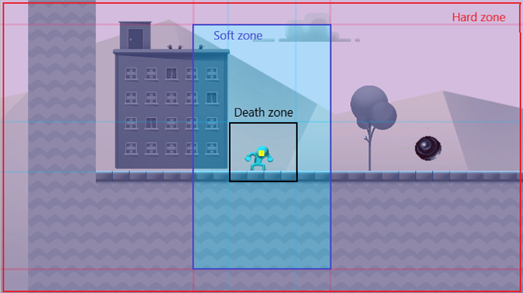
\includegraphics[scale=1]{Memoria/Aspectos_relevantes/Camaras/Camara_Cinemachine}
\caption{Distintas regiones que tiene en cuenta Cinemachine virtual camera.}
\end{figure}

A grandes rasgos Cinemachine virtual camera tiene en cuenta 4 cosas:
\begin{itemize}
\item
El objetivo a seguir (punto amarillo).
\item
La death zone (zona sin colorear).
\item
La soft zone (zona azul).
\item
La hard zone (zona roja).
\end{itemize}
El objetivo a seguir es el objetivo principal mencionado en la introducción. El objetivo principal es el objeto que se ha de mostrar en todo momento en cámara y que la Cinemachine virtual camera se encargará de mostrar por cámara siempre.\\
La death zone es la zona por la que se podrá mover el objetivo principal sin que la cámara se mueva. En cuanto el objetivo principal salga de la death zone la cámara se empezará a mover. El objetivo principal no es el objeto entero que se establece como objeto a seguir, sino el vector que representa su posición (se puede obtener mediante gameobject.transform.position), de manera que los límites del objeto pueden sí salirse de la death zone sin compromiso, pero solo mientras su posición que permanezca dentro de la death zone. Esto será así también para la soft zone y la hard zone.\\
Una vez el objetivo principal entre en la soft zone, la cámara comenzará a moverse hacia el objetivo principal hasta volver a meterlo en la death zone. La velocidad con la que la cámara persigue al objetivo principal depende de la distancia a la que este se encuentre (cuanto más lejos del centro de la cámara el objetivo principal, mayor será la velocidad de la cámara). El objetivo principal puede moverse por la soft zone sin que la cámara lo alcance mientras la cámara no tenga la velocidad necesaria para devolverlo a la death zone.
La hard zone es una zona por la que el objetivo principal no podrá desplazarse. En cuanto este alcance la hardzone, la cámara para devolver a la soft zone al objetivo principal. En realidad lo que hace la cámara es cambiar su posición a una en la que se encuentre el objetivo principal de la manera lo más consistente posible. Sinceramente, la Cinemachine virtual camera es bastante consistente a la hora de cambiar su posición a otra. Sin embargo, esta es la causa de uno de los dos problemas con los portales. Al cambiar la posición del objetivo principal a una que está en la hard zone, la cámara se mueve de una posición a otra sin hacer el recorrido que lleva de la posición anterior a la nueva, desorientando al jugador y haciendo que no sepa de donde ha venido.

Un sistema de gestión de cámara ideal sería uno que no posea hard zone, solo soft zone y death zone, de manera que al atravesar un portal la cámara también realice el recorrido de un portal a otro. A malas, este problema se puede solucionar haciendo que los portales no teletransporten al jugador de un punto a otro sino que simplemente lo muevan muy rápido. Esta puede ser una medida que se tome si no se logra aplicar el sistema gestor de cámaras deseado.

\subsection{Sistema de gestión de cámaras final}
El sistema de gestión de cámara que traía por defecto la plantilla de Platformer Microgame es la siguiente:

\clearpage
\begin{figure}[h]
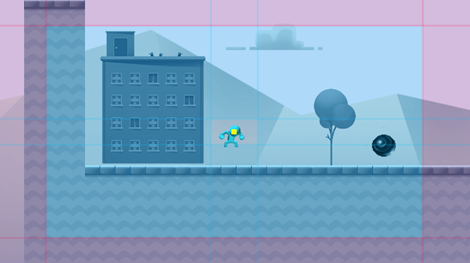
\includegraphics[scale=1]{Memoria/Aspectos_relevantes/Camaras/Cinemachine_Platformer_Microgame}
\caption{Sistema de gestión de cámaras de Platformer Microgames}
\end{figure}

Este sistema de cámaras tiene dos problemas principales: la vista de la cámara está demasiado cerca del personaje, dificultando al personaje ver lo que tiene alrededor y que dependiendo de la velocidad del jugador, es posible que la cámara no siga lo suficientemente rápido al jugador dificultando todavía más que el jugador tenga conocimiento de lo que tiene alrededor. El nuevo sistema de cámaras ha hecho dos cambios principales: alejar la visión de la cámara y reducir el rango de la soft zone. Alejar la visión se justifica por si sola. Reducir el rango de la soft zone permite que el avatar del jugador se encuentre siempre en el centro de la pantalla. De esta forma da igual la velocidad del jugador, que siempre se encontrará en el centro y contará con suficiente margen de pantalla para poder reaccionar a los elementos que surjan por los extremos de la pantalla.\\
Se han tomado otras dos decisiones adicionales. Una de ellas es aumentar la región ocupada por la death zone para que el jugador tenga una zona de estabilidad en la que no se mueve la cámara permitiéndole desplazarse con la estabilidad de que la cámara se mantenga estática y, adicionalmente, prepararle para el movimiento de la cámara, que no será tan brusco si el jugador ya se está moviendo frente a que la cámara empiece a moverse con el jugador.\\
La otra decisión ha sido desplazar la soft zone y la death zone un poco hacia la izquierda. Esta decisión se ha tomado con la intención de dar más espacio al jugador a ver lo que le viene desde la derecha. Esto se debe a que, en la mayoría de los casos, el lado izquierdo del mapa será conocido, mientras que el lado derecho es desconocido. Al tener conocimiento previo de lo que hay al lado izquierdo de la pantalla no hace falta tener visión absoluta del juego. Sin embargo, al encontrarse lo desconocido casi siempre en el lado derecho de la pantalla, se ha considerado recomendable mostrar más espacio al lado derecho de la pantalla que al izquierdo.

\begin{figure}[h]
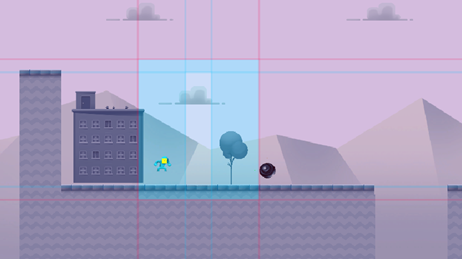
\includegraphics[scale=1]{Memoria/Aspectos_relevantes/Camaras/Camara_Cinemachine_juego}
\caption{Sistema de gestión de cámaras final aplicado}
\end{figure}

Ninguno de estos cambios solucionan el problema de los portales. Esto se debe a que, haciendo que la cámara siga la trayectoria entre portales, si los portales están a demasiada distancia (la principal razón para hacer que la cámara siga la trayectoria entre portales) el movimiento entre frames de la cámara es demasiado grande, desorientando al jugador más de lo que le ayuda a saber que camino ha recorrido. Se ha decidido solucionar este problema de otra forma, como por ejemplo dibujar líneas que conecten portales pareja.